\documentclass[12pt]{article}  
%%Read the manual for other options. 

\pagestyle{empty} %%Eliminates page numbers
%%\input rmb_macros
%%Collect your favorite macros in a 
%%separate file

%\input amssym.def
%\input amssym
%\input mssymb
%%Defines additional symbols



\usepackage{graphics}
\usepackage{amsmath,amssymb,amsthm, multicol,tikz,pgf,subfig,enumerate}
\usetikzlibrary{arrows.meta}
%\usepackage[pdftex]{graphicx}
\usepackage{epsf}
\newenvironment{theorem}
{\begin{proof}[Theorem]}
{\end{proof}}
%%Use to include pictures. 

%\newcommand{\comment}[1]{}
%\newcommand{\sobolev}[2]{W^{#1,#2}}
%\newcommand{\sobolev}[2]{L^#2_#1}
%%Some examples of macros or new commands.

%\addtolength{\oddsidemargin}{-.75in}
%\addtolength{\evensidemargin}{-.75in}
%\addtolength{\textwidth}{1.5in}
%\addtolength{\topmargin}{-1in}
%\addtolength{\textheight}{2.25in}
%%Set margins, defaults are ok. 

\begin{document}
% \begin{center}
% {\bf \Large Some Games}
% \vspace{0.2cm}
% \hrule
% \end{center}

\section*{A Tic-Tac-Toe-Like Game}
\begin{figure}[h]
	\centering
    \subfloat[Empty Board]{{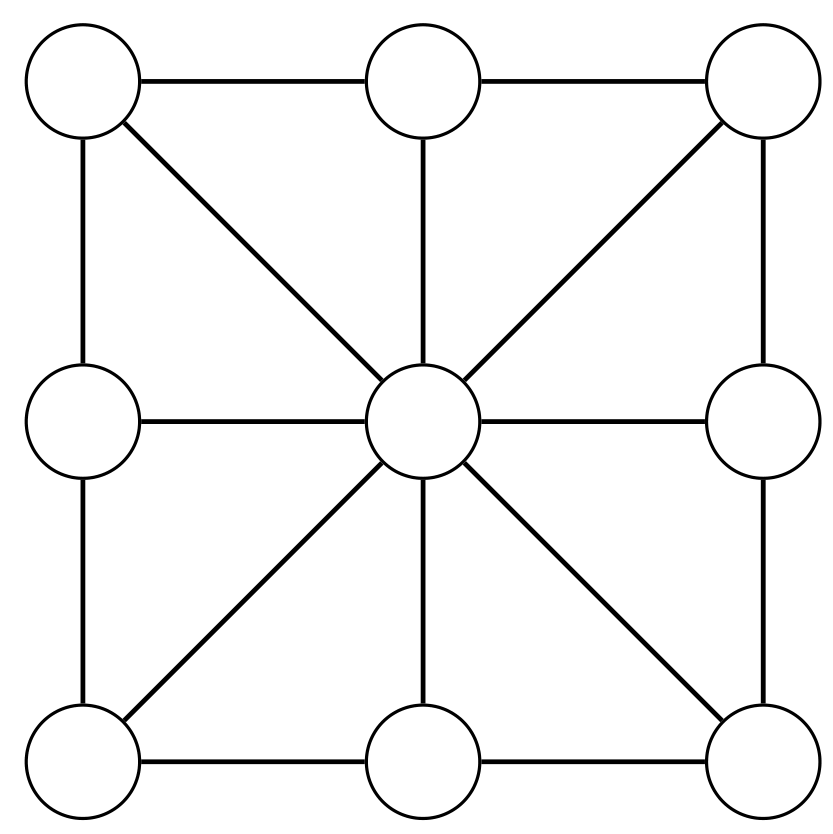
\includegraphics[scale=.2]{achi_empty} }}%
    \qquad
    \subfloat[Full Board]{{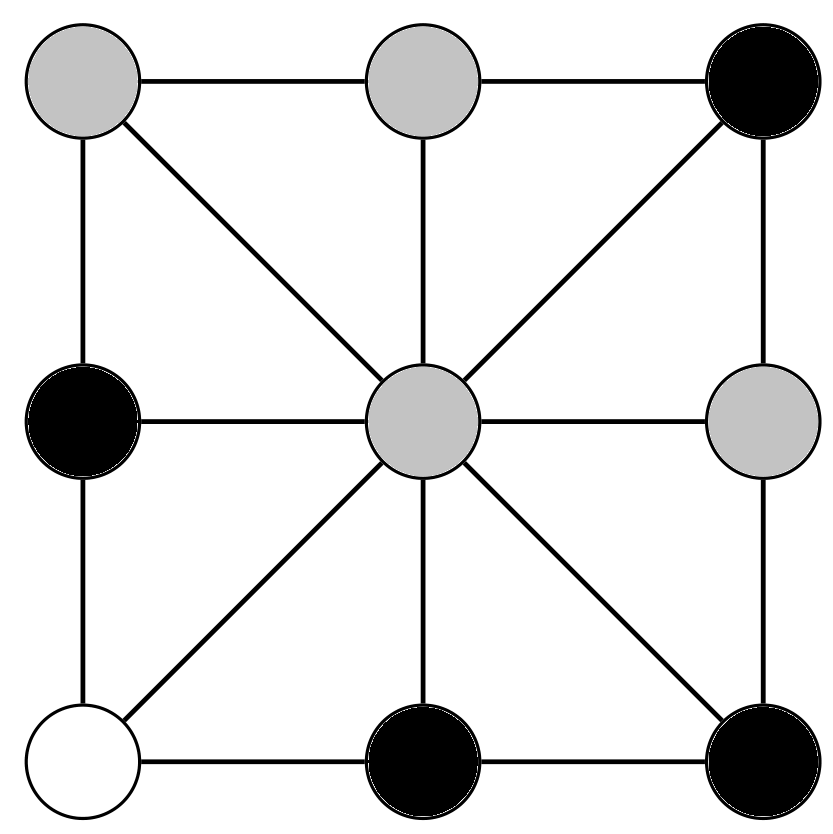
\includegraphics[scale=.2]{achi_full} }}%
    \\
    \subfloat[Gray's Next Move]{{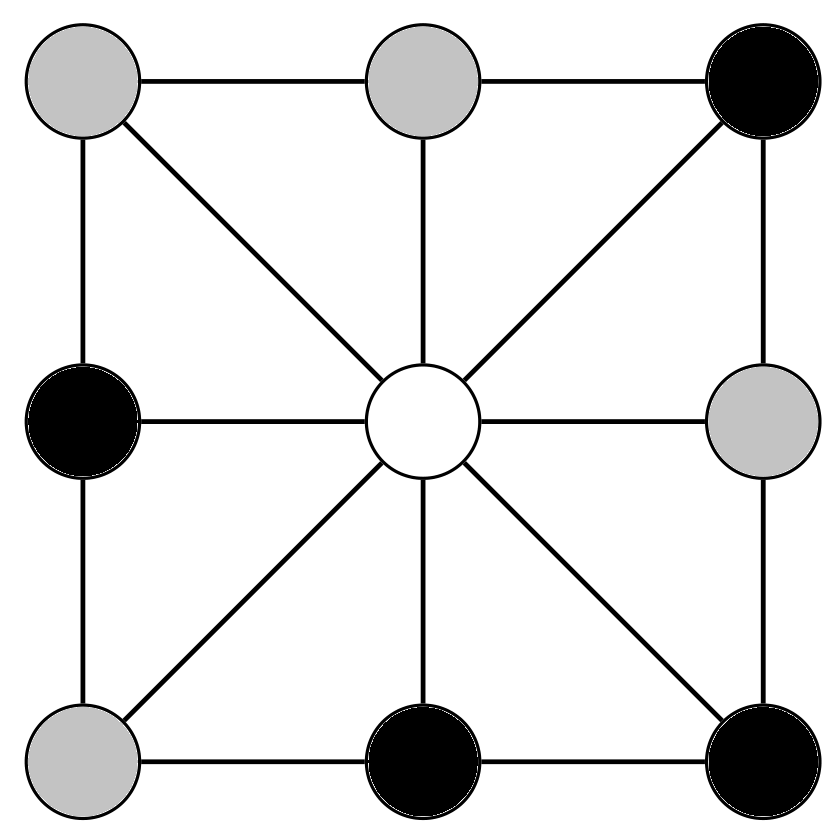
\includegraphics[scale=.2]{achi_next.png}}}
    \caption{}
    %\label{fig:example}%
\end{figure}
\noindent Two players start with four counters each. One player has gray counters, the other black. Just like in tic-tac-toe, this game is played on a three by three grid and players take turns placing their counters on the grid, trying to be the first to get three in a row.\\

\noindent Once both players have run out of counters, the players take turns sliding their already placed counters along the board's edges into the only empty space. Say the gray player goes first. The players go back and forth until they reach the sate shown in Figure 1(b). Neither player has three in a row yet, so play continues. Gray's only valid move is to slide their center counter the the lower-left space. Now black can move any of their counters to the center space. This continues until a player ends up with three counters in a row.\\

\noindent Play a few rounds of this game.

\subsection*{Questions}
\begin{enumerate}
	\item Is this game guaranteed to end?
	\vspace{4cm}
	\item Are any spaces on the board more valuable than others? Why or why not?
	\vspace{4cm}
	\item Does either player have an advantage? If so, can they be guaranteed to win with perfect play, regardless of what their opponent does?
\end{enumerate}

\newpage % CHOMP

\section*{A Counting Game}
This game involves two players. The first player chooses a positive integer less than or equal to 10. Then the second player adds a positive integer less than or equal to 10 to this first number. This goes back and forth, where the winner is whoever chooses a number so that the grand total is 101. Play a few rounds of this game.

\subsection*{Questions}
\begin{enumerate}
	\item Does either player have a winning strategy? What does it look like?
	\vspace{4cm}
	\item What if we adjust the numbers? Say the winning number is 77 and players take turns adding positive integers no greater than 8. What if the winning number is $N$ and players add positive integers no greater than $m$?
	\vspace{4cm}
	\item What if instead, whichever player is the first to bring the total to a number greater than or equal to 101 \textit{loses}? What's the strategy now?
\end{enumerate}

\newpage

\section*{Hex}
\begin{figure}[h]
	\centering
    \subfloat[Empty Board]{{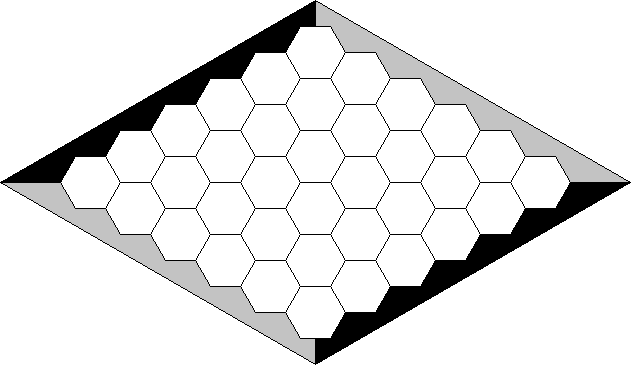
\includegraphics[scale=.3]{hex_empty} }}%
    \qquad
    \subfloat[A Few Moves In]{{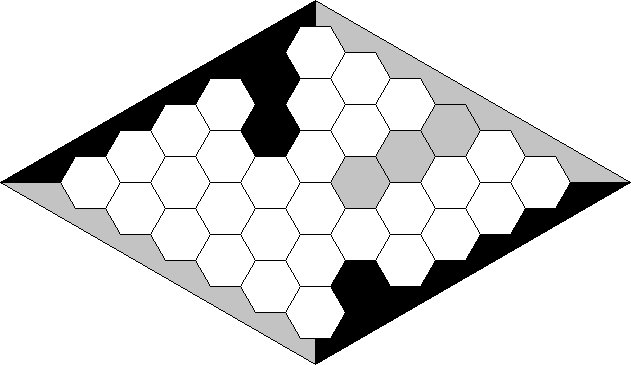
\includegraphics[scale=.3]{hex_progress} }}%
    \\
    \subfloat[Gray Wins!]{{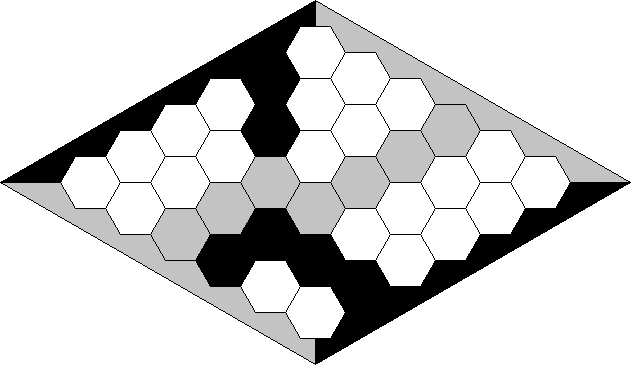
\includegraphics[scale=.3]{hex_end}}}
    \caption{}
    %\label{fig:example}%
\end{figure}
\noindent Hex is played with two players on a hexagonal grid. Each player has their own color, say gray or black. Players take turns coloring in hexagons with their assigned colors. Each player's goal is to build a connected path of their own color joining opposite sides of the board marked by their color. The first player to connect their sides wins. The four corner hexagons belong to both players.\\

\noindent Play some hex!


\subsection*{Questions}
\begin{enumerate}
	\item Let's show that Hex never ends in a draw.
	\begin{enumerate}[(a)]
		\item Say the game ends with a full board. Starting with a hexagon vertex at a corner, draw a path the edges between hexagons of different colors. Can this path intersect itself?
		\vspace{3cm}
		\item Why can't this path terminate on either side of the board (not counting corners)?
		\vspace{4cm}
		\item Why can't this path connect opposite corners?
		\vspace{4cm}
		\item Conclude that one player must have won.
		\vspace{4cm}
	\end{enumerate}

	\item Now that you know that somebody must win, can either player come up with a winning strategy?
\end{enumerate}




% \newpage
% \begin{tikzpicture}
% \begin{scope}[every node/.style={circle,thick,draw}, minimum size=1cm]
%     \node (v1) at (0,0) {};
%     \node (v2) at (0,3) {};
%     \node (v3) at (0,6) {};
%     \node (v4) at (3,0) {};
%     \node (v5) at (3,3) {};
%     \node (v6) at (3,6) {};
%     \node (v7) at (6,0) {};
%     \node (v8) at (6,3) {};
%     \node (v9) at (6,6) {};   
% \end{scope}

% \begin{scope}[every node/.style={fill=white,circle},
%               every edge/.style={draw=black,very thick}]
%     \path (v1) edge (v2);
%     \path (v2) edge (v3);
%     \path (v1) edge (v4);
%     \path (v3) edge (v6);
%     \path (v1) edge (v5);
%     \path (v4) edge (v5);
%     \path (v5) edge (v6);
%     \path (v3) edge (v5);  
%     \path (v2) edge (v5);  
%     \path (v4) edge (v7);  
%     \path (v5) edge (v8);  
%     \path (v5) edge (v7);  
%     \path (v5) edge (v9);  
%     \path (v6) edge (v9);  
%     \path (v7) edge (v8);  
%     \path (v8) edge (v9);  
% \end{scope}
% \end{tikzpicture}


\end{document}